% Impedanz-Ortskurve RLs-Glied
% R=var. mit R=p*R0, p in [0,3]
% wL=konst. mit wL=w0L0
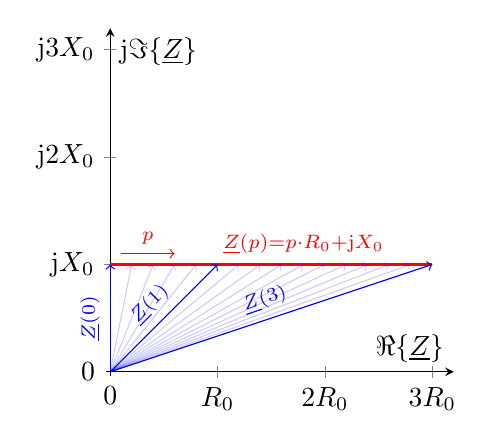
\begin{tikzpicture}
    \begin{axis}[
        xlabel=$\Re\{\underline{Z}\}$,
        ylabel=$\mathrm{j}\Im\{\underline{Z}\}$,
        axis lines=center,
        xmin=-0.2,xmax=16,% scaling: 5/1 = coordinates/shown values
        ymin=-0.2,ymax=16,% scaling: 5/1 = coordinates/shown values
        width=6cm, height=6cm,
        clip=false,
        xtick={0,5,10,15},% tick near center <0.01 not displayed
        xticklabels={,$R_0$,$2R_0$,$3R_0$},
        ytick={0,5,10,15},
        yticklabels={,$\mathrm{j}X_0$,$\mathrm{j}2X_0$,$\mathrm{j}3X_0$},
    ]
        % manual ticks at (0,0)
        \node[anchor=north,yshift=-2pt] at (0,0) {$0$};
        \node[anchor=east,xshift=-2pt] at (0,0) {$0$};
        % Ortskurve
        \addplot[mark=none,thick,red,domain=0:15] ({x},{5})
            node[pos=0.6,above,sloped]{$\scriptstyle\underline{Z}(p)=p\cdot R_0 + \mathrm{j}X_0$};
        % Richtungspfeil
        \addplot[->,red] coordinates{(0.5,5.5)(3.0,5.5)}
            node[midway,above]{$\scriptstyle p$};
        % Zeiger
        \foreach \i in {0,...,15}{\addplot[->,blue,opacity=0.2] coordinates{(0,0)({\i},5)};}
        \addplot[->,blue] coordinates{(0,0)(0,5)}   % Zeiger p=0
            node[midway,above,sloped]{$\scriptstyle\underline{Z}(0)$};
        \addplot[->,blue] coordinates{(0,0)(5,5)}   % Zeiger p=5
            node[midway,above,sloped]{$\scriptstyle\underline{Z}(1)$};
        \addplot[->,blue] coordinates{(0,0)(15,5)}  % Zeiger p=15
            node[midway,above,sloped]{$\scriptstyle\underline{Z}(3)$};
    \end{axis}
\end{tikzpicture}